\chapter{Title}
\section{Appendix}
\section{Detailed calculation of stationary moments}
In this section an expression for the $n^{\text{th}}$ stationary moment for the LRC model is derived.  The approach is analogous for the LES model and since the results are already known \cite{engen2000}, a detailed derivation isn't given, though one remark is made on the application of this method to diffusion processes.

\subsection{LRC model}

Before beginning, the chain rule for jump processes \cite{hansonBook} is stated without proof, for reference.  Let $X_t$ by a general process given by
\be
dX_t = f(X_t,t)dt + h(X_{t^-},t^-)dN_t
\ee

\noindent with $f$ and $h$ deterministic functions, $N_t$ a Poisson process with rate $\lambda$, and $t^-$ denoting the It\^{o} convention as in the main text.  Further let $Y_t \equiv F(X_t,t)$ be a transformed process.  Then $Y_t$ is governed by
\be
dY_t = \left(\partial_tF(X_t,t) + f(X_t,t)\partial_{X_t}F(X_t,t)\right)dt + \Delta Y_{t^-}^{jump}dN_t
\ee

\noindent with $\Delta Y_{t^-}^{jump} \equiv F(X_{t^-} + h(X_{t^-},t^-)) - F(X_{t^-},t^-)$.


Now recall the LRC model,
\be
dX_t = r X_t\left(1-\frac{X_t}{K}\right)dt  -(1-f)X_tdN_t.
\ee

\noindent The first step is to change variables to $X^n_t$ using the stochastic chain rule for jump SDEs.  The result is
\be
dX^n_t = nr X^n_t\left(1 -\frac{X_t}{K}\right)dt -(1-f^n)X^n_tdN_t.
\ee

\noindent Then, each term in this SDE is averaged.  The expectation of $X^n_{t^-}dN_t$ can be factored:  $\expec[X^n_{t^-}dN_t] = \expec[X^n_{t^-}]\expec[dN_t] = \expec[X^n_{t^-}]\lambda dt$.  Intuitively, this is because the two processes appear mutually independent.  The Poisson process has independent increments, and since the It\^{o} convention was used, $X^n_{t^-}$ is independent of $N_t$, which occurs in the future.  This is certainly true for a discrete time model, but care must be taken in the continuous limit.  

A more rigorous argument can be made using the Dominated Convergence Theorem.  The case $n=1$ is considered without loss of generality.  Consider $X_j$, a discrete partition of the continuous time process $X_t$, such that $X_j \to X_t$ in probability.  Then, sums of $X_j$ converge in probability to integrals, in particular,
\be
\sum_j X_{j-1} \Delta N_j \to \int_T X_{t^-} dN_t,
\ee

\noindent where $\Delta N_j$ is a partition of the Poisson process.  The Dominated Convergence Theorem says that if $X_t$ is dominated by an integrable function on the interval $T$,
\be
\expec\left [\sum_j X_{j-1} \Delta N_m\right] \to \expec\left[\int_T X_{t^-} dN_t\right]
\ee

\noindent in probability.  Since populations in the LRC model are bounded by the carrying capacity for all time, this is always valid.  The expectation of the sum is straightforward, leading to the result,
\be
\expec\left[\int_T X_{t^-} dN_t\right] = \int_T\expec[X_{t^-}]\lambda dt,
\ee

\noindent from which the infinitesimal version follows as a special case.

Factoring the expectation results in an ODE for the $n^{th}$ moment.  In the steady state, this becomes the recursion relation
\be
\expec[X^{n+1}] = K\left(1 - \frac{\lambda(1-f^n)}{nr}\right)\expec[X^{n}].
\ee

\noindent Defining 
\be
c_n \equiv \left(1 - \frac{\lambda(1-f^n)}{nr}\right),
\ee

\noindent the $n^{th}$ moment can be expressed in terms of the mean as
\be
\expec[X^n] = K^{n-1}\left(\prod^{n-1}_{m=1}c_m \right)\expec[X].
\ee

To complete the recursion relation, the mean must be computed independently.  This is accomplished by changing variables to $\ln X_t$ using the chain rule for jump processes:
\be
d\ln X_t = r\left(1 -\frac{X_t}{K}\right)dt +\ln f dN_t,
\ee

\noindent which in the steady state gives an expression for the stationary mean,
\be
\expec[X] = K\left(1 + \frac{\lambda}{r}\ln f\right).
\ee

\noindent Plugging this back into equation (A10) gives the final result
\be
\expec[X^n] = K^{n}\left(1 + \frac{\lambda}{r}\ln f\right)\prod^{n-1}_{m=1}\left(1 - \frac{\lambda(1-f^m)}{mr}\right).
\ee

\noindent Evaluating this equation for $n=2$ leads to the expression for the variance in the main text:
\be
\Var[X]_{LRC} = K^2\frac{\lambda}{r}\left(-\ln f-(1-f)\right)\left(1+\frac{\lambda}{r}\ln f\right).
\ee

\subsection{LES model}
The derivation is analogous for the LES model, except that It\^{o}'s chain rule for diffusion processes is used.  Since the results are already known \cite{engen2000}, derived with traditional methods, a detailed computation will not be given.  However, one remark worth making concerns the expectation of $X_{t^-}dB_t$.  The intuitive argument outlined for the LRC model - that since the It\^{o} convention was employed the expectation of the product can be factored - gives the correct answer in this case, but is in fact not generally valid.  Essentially, for processes governed by equations of the form 
\be
dX_t = f(X_t,t)dt + g(X_{t^-},t^-)dB_t,
\ee

\noindent the integral $\int g(X_{t^-},t^-)dB_t$ can acquire non-zero expectation if the function $g$ grows too quickly.  A classic example is the CEV model of quantitative finance \cite{linetsky2010constant}, which is of the form $f(X_t,t) = X_t$ and $g(X_t,t) = X^{\gamma}_t$ for $\gamma > 1$.  However, one can use the fact that the exponential version of the LES model, i.e. $K \to \infty$, is a well known SDE for which $\expec\left[\int X_{t^-}dB_t\right]=0$.  This model is known as Geometric Brownian Motion and describes asset prices in the Black-Scholes model of quantitative finance \cite{linetsky2010constant}.  Since paths of the exponential model almost surely dominate paths of the LES model, $\int X_{t^-}dB_t$ for the LES model inherits the martingale property from the exponential case, which implies zero expectation.

Following the same procedure as for the LRC model, factoring expectations of $X^n_{t^-}dB_t$, results in

\be
\expec[X^n]_{LES} = K^{n}\left(1-\frac{\sigma^2}{2r} \right)\prod^{n-1}_{m=1}\left(1+\frac{(m-1)\sigma^2}{2r} \right).
\ee

\noindent Special cases of this include

\be
\expec[X]_{LES} = K\left(1-\frac{\sigma^2}{2r}\right)
\ee

\noindent and

\be
\Var[X]_{LES} = \frac{K^2\sigma^{2}}{2r}\left(1-\frac{\sigma^2}{2r}\right).
\ee



\section{The diffusion limit and the Central Limit Theorem}

This section contains details of the construction of the LES model from the LRC model in the limit of infinitely frequent, infinitesimal catastrophes, referred to here as the diffusion limit.  The complete transformation involves all four LRC model parameters and is specified as follows.  Let $\alpha$ be a scale parameter, $LRC(r,K,\lambda,f)$ an LRC model, and $\sigma$ be the target noise-strength parameter of the limiting LES model.  Fix $\lambda\ln^2 f = \sigma^2$, and scale
\begin{equation*}
\lambda' = \alpha \lambda,\text{\hspace{.4cm}}\ln f' = -\sigma/\sqrt{\lambda'}
\end{equation*}
\begin{equation*}
r' = r\left(1- \frac{\lambda'\ln f'}{r}\right) = r\left(1+ \frac{\sigma\sqrt{\lambda}}{r}\sqrt{\alpha}\right),
\end{equation*}
\begin{equation}
K' = K\left(1  -\frac{\lambda'\ln f'}{r}\right) = K\left(1+ \frac{\sigma\sqrt{\lambda}}{r}\sqrt{\alpha}\right).
\end{equation}


\noindent The claim is that in taking the limit $\alpha \to \infty$, the LRC model $LRC(r',K',\lambda',f')$ gets mapped to an LES model $LES(r_{ES},K_{ES},\sigma)$, with $\sigma^2 = \lambda\ln^2f$, $r_{ES} = r(1+(2r)^{-1}\sigma^2)$, and $K_{ES} = K(1+(2r)^{-1}\sigma^2)$, such that the stationary means of both models are equal. I first motivate the form of this transformation, which involves all four LRC model parameters, by studying the behavior of the stationary moments.  I then show how the precise form of these limits, namely $\lambda\to\infty$, $f\to 1$, such that $\lambda\ln^2f\to$ const., follows from functional generalizations of the Central Limit Theorem (CLT), in which a scaled, compensated Poisson process limits to Brownian motion.  Finally, I show analytically how the full transformation maps the LRC model into the LES model.  

\subsection{Motivation}

As discussed in the main text, taking the limits $\lambda\to\infty$, $f\to 1$, such that $\lambda\ln f\to$ const. is analogous to the law of large numbers, leading to a deterministic limit.  The correct limits instead are $\lambda\to\infty$, $f\to 1$, such that $\lambda\ln^2f\to$ const., which I show below is analogous to the CLT.  To motivate the final four parameter transformation, let us first consider the behavior of the LRC variance under these limits:

\bea
\Var[X] &=& K^2\frac{\lambda}{r}(-\ln f -(1-f))\left(1+\frac{\lambda}{r}\ln f\right)\nonumber\\ 
&\xrightarrow{\text{limits}}&K^2\frac{\lambda \ln^2 f}{2r}\left(1+\frac{\lambda}{r}\ln f\right)\nonumber\\
&=&  K^2\frac{c^2}{2r} -K^2\frac{c^3}{r^2}\sqrt{\lambda}.
\eea
\noindent with $c = \text{ const } = -\sqrt{\lambda}\ln f$.  In taking the limit $f\to1$, the relation $(-\ln f -(1-f)) \to 2^{-1}\ln^2f$ was used, based on a $2^{\text{nd}}$ order Taylor expansion.  

The variance diverges, but a part of it remains finite.  The finite piece of the variance in this limit is exactly the variance of an LES model with $\sigma^2 = \lambda\ln^2 f$ and increased growth parameters $K_{ES} = K(1+(2r)^{-1}\sigma^2)$, and $r_{ES} = r(1+(2r)^{-1}\sigma^2)$.  Looking at the behavior of the mean in this limit leads to the same conclusion.  This suggests that this limit does take the LRC model into an LES model, but one that is accompanied by a noise-induced drift that diverges as $\sqrt{\lambda}$.  This is divergence should be expected, as it reflects the unidirectionality of jumps in the LRC model, which is absent in the LES, analogous to the divergence of the mean of a Poisson distribution when it limits to a Gaussian.  To obtain a non-trivial limiting process, this drift needs to be subtracted off, for example, by adding a term $-\lambda\ln f dt$ to the LRC model SDE.  This is equivalent to rescaling the growth rate and carrying capacity each by a factor of $(1-r^{-1}\lambda\ln f)$, leading to the full four parameter transformation.


\subsection{Functional Central Limit Theorems}

The form of the limits  $\lambda\to\infty$, $f\to 1$, such that $\lambda\ln^2f\to$ const., is a direct consequence of the CLT.  The classical CLT says that given a set of $n$ random variables, $\{\xi_j\}$, that are identically and independently distributed (i.i.d.) with mean $\mu$ and finite variance $\sigma^2$, the sum of the deviations of these variables from their mean, when rescaled by $\sqrt{n}$, tends in distribution to a Gaussian variable as $n\to\infty$:

\be
\lim_{n\to\infty}\frac{\sum_j\xi_j -n\mu}{\sqrt{n}} = \eta \sim \mathcal{N}(0,\sigma^2)
\ee

\noindent where $\mathcal{N}(\mu,\sigma^2)$ is a Gaussian distribution with mean $\mu$ and variance $\sigma^2$.  The condition that the variables $\xi_j$ follow identical distributions can be relaxed, but we focus on this restricted case here.  

A vast body of mathematical literature concerns the construction of generalization of the CLT to stochastic processes.  One important generalization, which we will employ in the study of the Poisson process, is Donsker's theorem \cite{jacod2013limit}.  Donsker's theorem dictates the limit of a sequence of stochastic process, $X^{(n)}_t$, constructed from sums of i.i.d. random variables $\tilde{\xi}_j$ with zero mean and finite variance via

\be
X^{(n)}_t \equiv \frac{1}{\sqrt{n} }\sum_{j=1}^{[ns]}\tilde{\xi}_j\text{, \hspace{.2cm}}ns \equiv t.
\ee

\noindent Here we have introduced time as multiples of a unit $s$, such that $t = ns$, and $[...]$ denotes the integer part.  Donsker's theorem says that as $n\to\infty$ with $s\to 0$ such that $ns\to t$ for arbitrary $t$, the processes $X^{(n)}_t$ converge in law to Brownian motion,
\be
X^{(n)}_t \to B_t.
\ee

\noindent Donsker's theorem can be used to show the convergence of the compensated Poisson process to Brownian motion in particular limits.  The idea is to write the Poisson process as a sum of intervals which themselves are i.i.d. random variables that meet the criteria for Donsker's theorem, and then scale the jump size and rate in the ways that map onto the $n\to\infty$ limit.  This approach is based on a method known as finite dimensional convergence, which is only applicable to processes with independent increments \cite{jacod2013limit}.  

Consider breaking a scaled, compensated Poisson process, $\epsilon \tilde{N}_t$ into a sum of finite intervals,


\be
\epsilon \tilde{N}_t = \epsilon\sum_{j=1}^{[ns]}\Delta \tilde{N}_j.
\ee


\noindent From inspection, we see that the appropriate mapping is $\lambda \to n\lambda$, $\epsilon = \sigma\lambda^{-1/2}$, in which case

\be
\epsilon \tilde{N}_t = \sigma\sum_{j=1}^{[ns]}\frac{\Delta \tilde{N}_j/\sqrt{\lambda}}{\sqrt{n}}.
\ee

\noindent  Donsker's theorem can then be applied with $\tilde{\xi}_j \equiv \Delta \tilde{N}_j/\sqrt{\lambda}$, resulting in

\be
\epsilon \tilde{N}_t  \xrightarrow{\lambda \to \infty, \text{ } \epsilon \to 0} \sqrt{\lambda}\epsilon B_t.
\ee

In the LRC model, collapse size is forced to zero by taking $f\to 1$.  This still leaves room for how exactly $\lambda$ and $f$ should map on to $\sigma$.  One choice would be to take $\epsilon = -(1-f)$, such that $\sigma^2 = \lambda (1-f)^2$.  In this case, a quick calculation shows that the limiting process would be an LES model with unchanged growth parameters, $(r,K)$, and consequently a reduced stationary mean of $K(1-(2r)^{-1}\sigma^2)$, whereas the original LRC process, after removing the divergence of $\lambda\ln f$, has a stationary mean of $K$.  Alternatively, one could take  $\epsilon = \ln f$, such that $\sigma^2 = \lambda \ln^2f$.  This is the case examined above, which results in an LES model with an unchanged stationary mean, but altered growth parameters.  Since our present goal is to normalize the effect of noise to construct a fair comparison of extinction risk, the latter choice is more appropriate.


\subsection{Convergence of LRC to LES}

I now discuss the convergence of the LRC model to the LES model via the convergence of the Poisson process to Brownian motion discussed above.  General conditions for the convergence of a pure jump Markov process to a diffusion are given in \cite{jacod2013limit}.  Rather than verify these general conditions here, I'll take a more intuitive approach that exploits the simplicity of the present models and uses the fact that both the LRC model and the LES model possess unique, strong solutions, as follows from special cases of a general result derived in \cite{bao2011competitive}.  This allows us to uniquely define a sequence of processes $X'_t(\alpha) \equiv F[\tilde{N}_t(\alpha); r(\alpha),K(\alpha),\lambda(\alpha),f(\alpha)]$, where $F$ is the solution to the LRC model depending on parameters $r$, $K$, $\lambda$, and $f$, and the limit of the sequence $X^*_t \equiv \lim_{\alpha\to\infty} X'_t(\alpha)$.   Existence and uniqueness of solutions to both models allows us in principle to take the limit and then invert the solution, recovering a diffusion SDE.  In practice, we can take the limit directly in the context of the LRC model SDE.  
To begin, recall the LRC model,
\be
dX_t = r X_t\left(1-\frac{X_t}{K}\right)dt -(1-f)X_{t^-}dN_t.
\ee

\noindent Let us expand $(1-f)$ in powers of $\ln f$ to second order and write the Poisson process in terms of its mean and compensated process.

\be
dX_t = r X_t\left(1-\frac{X_t}{K}\right)dt +\left(\ln f + \frac{1}{2}\ln^2f\right)X_{t}\lambda dt +\left(\ln f + \frac{1}{2}\ln^2f \right)X_{t^-}d\tilde{N}_t + \mathcal{O}(\lambda\ln^3f)
\ee

\noindent Now let us absorb the mean drift of the Poisson process as scaling factors for the growth rate and carrying capacity

\begin{multline}
dX_t = r \left(1+\frac{\lambda}{r}\ln f + \frac{\lambda}{2r}\ln^2f \right)X_t\left(1+\frac{X_t}{K\left(1-\frac{\lambda}{r}\ln f+ \frac{\lambda}{2r}\ln^2f \right)}\right)dt \\ 
+\left(\ln f + \frac{1}{2}\ln^2f \right)X_{t^-}d\tilde{N}_t + \mathcal{O}(\lambda\ln^3f).
\end{multline}

Now we apply the transformation [19] with $\alpha$ finite and evaluate $r'$ in terms of $r$ and $K'$ in terms of $K$.  This has the effect of canceling all $\lambda\ln f$ terms, as intended.

\begin{multline}
dX'_t(\alpha) = r \left(1 + \frac{\lambda'}{2r}\ln^2f' \right)X'_t\left(1-\frac{X'_t}{K\left(1 + \frac{\lambda'}{2r}\ln^2f' \right)}\right)dt \\
+\left(\ln f' + \frac{1}{2}\ln^2f' \right)X'_{t^-}d\tilde{N'}_t + \mathcal{O}(\lambda\ln^3f)
\end{multline}

\noindent where primed variables depend on $\alpha$.  Before taking the $\alpha\to\infty$ limit, we can identify $\lambda'\ln^2f'$ as $\sigma^2$, a finite constant independent of $\alpha$,

\be
dX'_t(\alpha) = r \left(1 + \frac{\sigma^2}{2r}\right)X'_t\left(1-\frac{X'_t}{K\left(1 + \frac{\sigma^2}{2r} \right)}\right)dt +\left(\ln f' + \frac{1}{2}\ln^2f' \right)X'_{t^-}d\tilde{N'}_t + \mathcal{O}(\lambda\ln^3f).
\ee

\noindent We can now evaluate the $\alpha\to\infty$ limit, knowing how $\tilde{N}_t$ transforms:  $\ln f'd\tilde{N}_t\to\sigma dB_t$ in law, $\ln^2 f'd\tilde{N}_t\to 0$, resulting in

\be
\lim_{\alpha\to\infty}dX'_t(\alpha) = dX^*_t = r \left(1 + \frac{\sigma^2}{2r}\right)X^*_t\left(1-\frac{X^*_t}{K\left(1 + \frac{\sigma^2}{2r} \right)}\right)dt +\sigma X^*_{t^-}dB_t.
\ee

The limiting process is an LES model with increased growth parameters $r_{LES} = r(1+(2r)^{-1}\sigma^2)$ and $K_{LES} = K(1+(2r)^{-1}\sigma^2)$.  Comparing this model to the transformed LRC model of [31] using the analytic results for the stationary mean equations (A12) and (A17) reveals that the two models do indeed have the same stationary mean.


\section{An alternative mapping that equates stationary means}

The stationary means of the LRC and LES models can also be equated by using the same growth rate and carrying capacities and mapping $\sigma^2 = -2\lambda\ln f$, as is clear from equations (A12) and (A17).  This mapping provides an alternative method of quantitatively comparing the two models, though one that is perhaps less meaningful than the diffusion limit approach.  It can be understood intuitively by plotting the time evolution of the mean population of both models in the presence and absence of extinction (Supplementary Figure 2A).  In the absence of extinction, both models asymptote to the same value.  In the presence of extinction, the LRC model average decays to zero faster than the LES model average, indicating higher extinction risk.  Computed directly, the mean times to extinction for the LRC model are significantly shorter than for the LES model (Supplementary Figure 2B), supporting the conclusions of the diffusion limit-based method.


\newpage
\section{Supplementary Figures}
%\renewcommand\thefigure{S1}  
\renewcommand\thefigure{S\arabic{figure}}  
\setcounter{figure}{0}    
\begin{figure}[h]
	\centerline{
		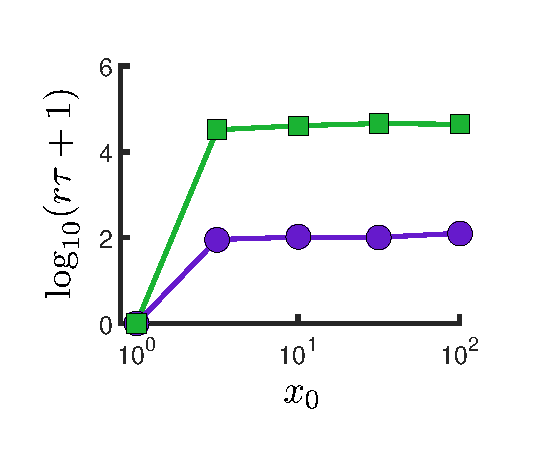
\includegraphics[width =3.25 in]{math/figureS1}}
	\caption{\textbf{Mean time to extinction is largely independent of initial starting population}.}  {Mean time to extinction, $\tau$, plotted on a shifted log scale as a function of initial starting population, $x_0$.  Green squares denote the LES model, purple circles denote the LRC model.  The mean extinction time, defined as the first hitting time to $x^* = 1$, starts from 0 but rapidly increases to a value independent of $x_0$.  Parameters:  $r = 1$, $K = 10^4$, $\lambda = .1$, $f = .01$, $N_{trials} = 500$.}
\end{figure}

%\newpage
%\renewcommand\thefigure{S2}    
\begin{figure}[h]
	\centerline{
		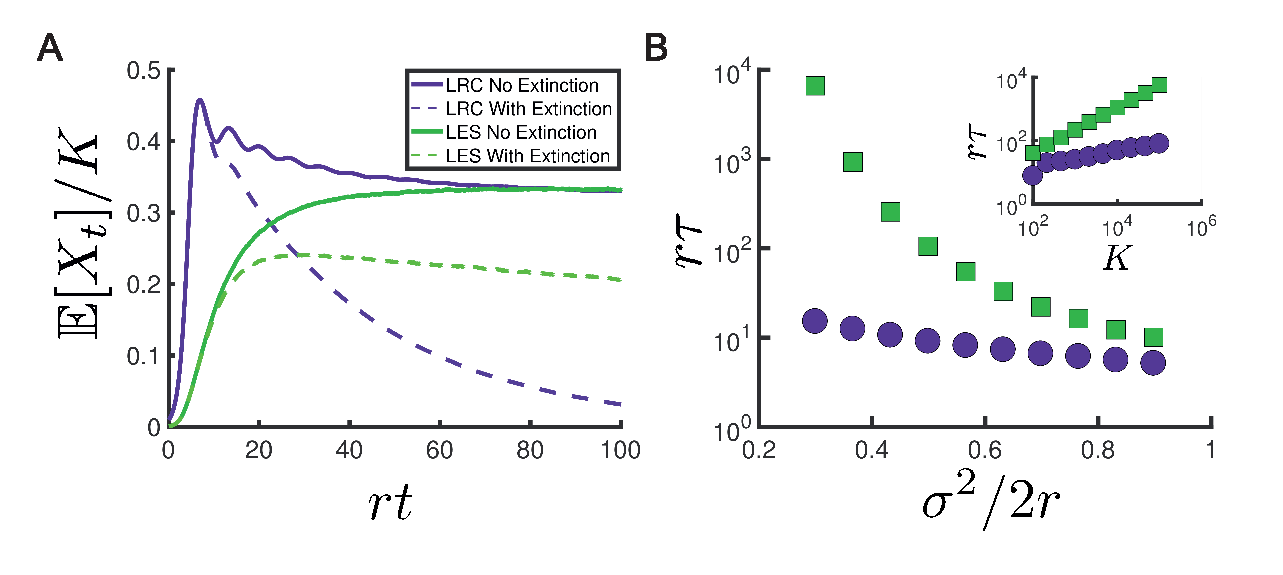
\includegraphics[width = 6.5 in]{math/figureS2}}
	\caption{\textbf{The LRC model has higher extinction risk than the LES model for equivalent stationary means.}} {\textbf{A:} Illustration of the mapping.  Numerical results for the average population plotted over time in the LRC (purple) and LES (green) models, showing both the cases of no extinction (dark solid lines) and extinction (light dashed lines) via an absorbing state at $x^* = 1$.  LES model has the same growth rate and carrying capacity as the LRC model and $\sigma$ is determined by $\sigma^2 = -2\lambda\ln f$, such that the two models have equal stationary means (Appendix C).  Parameters:  $r = 1$, $K = 10^4$, $\lambda = .1$, $f = .0012$, $\sigma = 1.16$, $dt = .01$, $N_{trials} = 5\cdot 10^5$.  \textbf{B:}  Mean time to extinction, $\tau$, in units of inverse growth rate, for LRC (purple circles) and LES (green squares) models as a function of noise strength, with $\sigma^2 = -2\lambda\ln f$.   Parameters:  $r = 1, dt = .01, N_{trials} = 5\cdot 10^3$.  For LRC model, $f = .01$ and $\lambda$ was varied from $.065$ to $.195$.  Inset:  Mean time to extinction as a function of carrying capacity.  Parameters:  $r = 1$,  $\lambda = .13$, $f = .01$, $\sigma = 1.09$, $dt = .01$, $N_{trials} = 5\cdot 10^3$.}
\end{figure}

\renewcommand\thefigure{\arabic{figure}}    
